\documentclass[11pt,a4paper, english, swedish
]{article}
\pdfoutput=1

\usepackage{custom_as}
\usepackage{multirow}

\graphicspath{ {fig_and_code/} }

%%Drar in tabell och figurtexter
\usepackage[margin=10 pt]{caption}
%%För att lägga in 'att göra'-noteringar i texten
\usepackage{todonotes} %\todo{...}

%%För att själv bestämma marginalerna. 
\usepackage[
            top    = 3cm,
%            bottom = 3cm,
%            left   = 3cm, right  = 3cm
]{geometry}

%%För att ändra hur rubrikerna ska formateras
%\renewcommand{\thesection}{...}

\newcommand{\Thalv}[2]{\ensuremath{}T_{\nicefrac{1}{2}}\left(^{#1}\text{#2}\right)}

\newcommand{\A}{\ifmmode\upalpha\else$\upalpha$\fi}
\newcommand{\BM}{\ifmmode\upbeta^{\!-}\else$\upbeta^{\!-}$\fi}
\newcommand{\G}{\ifmmode\upgamma\else$\upgamma$\fi}


\begin{document}


%%%%%%%%%%%%%%%%% vvv Inbyggd titelsida vvv %%%%%%%%%%%%%%%%%

\title{K6 -- neutronaktivering av silver}
\author{Andréas Sundström}
\date{\today}

\maketitle

%\begin{abstract}
%\end{abstract}
%%%%%%%%%%%%%%%%% ^^^ Inbyggd titelsida ^^^ %%%%%%%%%%%%%%%%%

%Om man vill ha en lista med vilka todo:s som finns.
%\todolist

\section{Inledning}
I den här labben studeras neutronaktivering av silver. Detta bygger på att de två naturligt förekommande silverisotoperna $^{107}\text{Ag}$ och $^{109}\text{Ag}$ kan omvandlas till $^{108}\text{Ag}$ respektive $^{110}\text{Ag}$ genom neutroninfångning.

Rapporten börjar med att studera effekten från olika neutronenergier. Detta görs genom att dels undersöka siverisotopernas tvärsnitt för termiska neutroner ($E\sim \unit[10]{meV}$), dels undersöka påverkan från olika mycke bromsning med hjälp av parafin. De termiska neutronera undersöks genom att klä in silvret i kadmium som har ett mycket stort tvärsnitt för termiska neutroner. 

Därefter undersöks de två producerade silverisotopernas halveringstider. Detta görs genom att mäta aktiviteten och studera hur den varierar i tiden.

\section{Metod}
Silvret först behöver neutronaktiveras, men då behöver neutronera bromsas till rätt energier för att silverkärnorna effektivt ska kunna ta upp netronerna. De båda natuligt förekommande silverisotoperna har, för neutronenergier lägre än ca 1\,eV, ett tvärsnitt som beror inverst mot neutronenergin~\cite{labPM}. Över 1\,eV börjar båda isotoperna komma in i sina resonansregioner, där varierar tvärsnittet mycket kraftigt med många distinkta toppar~\cite{labPM}. 

Det vore alltså teoretiskt önskvärt att få så låga neutronenergier som möjligt för att få ett så stort tvärsnitt som möjligt. Detta kan till viss mån testat kvalitativt i den här labben, vilket görs genom att undersöka olika kraftig bromsning av neutronerna. 

För att bormsa neutronerna används framför allt väte; i den här laborationen användes parafin, som är stora kol-vätekedjor, för att bromsa neutronerna. Man använder väte för att neutroner och protoner har ungefär samma massa, vilket gör att en stor andel av neutronens rörelsemängd kan överföras till protonen vid en kollision. 

\subsection{Uppställning}
Uppställningen bestod av en neutronkälla, en silverplatta på en pinne, ett kadmiumskal till silverplattan och en behållare med parafin runt neutronkällan som har tre positioner att sätta in silverplattan.

Neutronkällan består av en fin blandning av beryllium och radium. När radiumet sönderfaller emitteras en \A-artikel som kan fångas upp av en beryliumkärna, vilket ger en neutron och en kolkärna. Allt enligt
\begin{equation}
^9_4\text{Be} + \A \to \text{n} + ^{12}_{\phantom{1}6}\!\text{C}^*.
\end{equation}
Den exciterade kolkärnan kommer att emittera en \G, men det är inte intressant för den här laborationen. Det viktigaste är att det producreas en neutron som sedan kan fångas upp av sivret.

I \figref{fig:aktivering} visas de tre positionerna som silverplattan kan placeras i förhållande till neutronkällan. Utrymmet mellan neutron källan och position 2 och 3  finns parafin. Genom att placera silverplattan i någon av positionerna kan effekten från olika mycket bromsande parafin undersökas.

Vidare visar även \figref{fig:aktivering} att en lika stor platta kommer att uppta en mindre rymdvinkel, sett från neutronkällan, ju längre bort man placerar den. För att detta inte ska påverka resultaten för neutronenergierna måste denna variation i rymdvinkel korrigeras. Detta görs genom att betrakta neutronkällan som en punktkälla placerad i mitten; därefter används att rymdvinkeln minskar (ungefär) kvadratiskt med avståndet. Tillsammans kan man enkelt beräkna en korrektionsfaktor 
\begin{equation} \label{eq:k}
k_i=\left(\frac{r_i}{r_1} \right)^2
\end{equation}
som används så att mätningar i alla lägen korrigeras så att de motsvarar en rymdvinkel som i läge~1.

\begin{figure}\centering
\resizebox{.5\textwidth}{!}{\input{fig_and_code/aktivering.pdf_t}}
\caption{De tre olika positionerna där en silverplatta kan placeras i förhållande till neutronkällan. 
För att bara mäta effekten från olika mycket parafin måste man kompensera för att en lika stor platta på större avstånd tar upp en mindre rymdvinkel. Alltså att färre antal neutroner kommer att träffa plattan som är längre bort.}
\label{fig:aktivering}
\end{figure}


\subsection{Mätningar}
Först gjordes en bakgrundsmätning för att veta hur mycket bakgrundsstrålning som fångades upp av geigermätaren. Detta gjordes för att korrektionsfaktorn $k$ kan bli ganska stor, men bakgrunden kommer inte att påverkas av var man placerade silvret. 

Därefter mättes aktiviteten från de olika positionerna, med och utan kadmiumskalet (dock inte med kadmiumskalet i pos.~1 då det är förtrångt där för att få plats med skalet). Detta kom att ge information om vilken typ av neutroner som har högst tvärsnitt hos silvret. Dessa mätningar gjordes genom att aktivera silvret under 2,5~minuter i de olika positionerna, och sedan räkna antalet sönderfall i tidsintervaller 30--60\,s efter att aktiveringen avslutats. 

Med informationen om vilken position som gav den effektivaste neutroninfångningen kunde sedan silvret placeras där för att aktiveras. När silvret sedan hade aktiverats under ca 10~minuter mättes hur dess aktivtet förändrade sig i tid. Från den informationen kan sedan den initiala andelen av de olika isotoperna samt deras halveringstid bestämmas. Aktiviteten mättes genom att räkna antalet sönderfall i olika givna tidsintervall. 

\subsubsection{Misstag i mätningen}
På grund av en miss i tidtagningen den första gången silvret skulle aktiveras överaktiverades silvret. Då var vi tvungna att vänta på att radioaktiviteten skulle avta tillräckligt för att göra om mätningarna. 

Sedan fortsatte problemen med att kadmiumskalet verkade ha glidit upp när mätningen i position~3 ''med kadmium''. Detta upptäcktes tyvärr inte förrän efter aktiveringen var gjord, men på grund av tidsbrist från den första missen kunde inte mätningen göras om som önskat. Detta gör att resultatet för ''Utan kadmium, Pos. 3'' i \tabref{tab:aktivitet} troligen inte är tillförlitligt. 


\subsection{Databehandling} \label{sec:databehandling}
\paragraph{Neutronenergi}
Vid mätningarna av olika neutronenergiers påverkan gjordes korrigeringar för bakgrunden och rymdvinkeln. Rymdvinkelkorrigeringen gjordes genom att multiplicera det bakgrundskorrigerade aktivitetsvärdet med $k$ från \eqref{eq:k}.

\paragraph{Halveringstider}
För att beräkna beräkna halveringstiderna behöver man anpassa två exponentialsamband till akrivitetskurvan. Detta eftersom 
\begin{equation}
A_\text{tot}(t) = A_{1}(t) + A_{2}(t) 
= A_{1}(0)\ee^{-\lambda_1 t} + A_{2}(0)\ee^{-\lambda_2 t},
\end{equation}
där $A_1$ och $A_2$ samt $\lambda_1$ och $\lambda_2$ är de olika isotopernas aktivtet respektive sönderfallskonstant. Notera att det inte, utan extra information, går att ta fram vilken av de faktiska isotoperna som hör till index 1 respektive 2. 

För att kunna göra anpassningarna utnyttjas att $\lambda_1\neq\lambda_2$. Eftersom det är godtyckligt vilken isotops om har vilket index kan vi välja $\lambda_1>\lambda_2$. Detta betyder att $A_{1}(t)\ll A_{2}(t)$ vid stora tider. Detta borde då synas som att $A_\text{tot}\approx A_2$ blir linjär i en logplot för stora~$t$. Därifrån kan $A_2(0)$ och $\lambda_2$ bestämmas genom en linjäranpassing till logaritmen av $A_\text{tot}$ för stora~$t$. 
Sedan använder man att $A_1=A_\text{tot}-A_2$ för att på samma sätt bestämma $A_1(0)$ och $\lambda_1$.



\section{Resultat och Diskussion}

I \tabref{tab:aktivitet} visas de uppmätta aktiviteterna från silvret som hade aktiverats i de olika positionerna med och utan kadmiumskalet. Efter korrigering mot bakgrunden (som visade sig vara mycket liten) och rymdvinkel syns att kadmiumskalet ser ut att effektivt ha blockerat\footnotemark{} aktiveringen av silvret. I position~2 syns en mer än 4~gångers skillnad mellan att ha skalet på respektive av.
\footnotetext{Se avsnittet ovan, om misstag i mätningen, varför tabellvärdet för ''Utan kadmium, Pos. 3'' bör bortses ifrån.}

Eftersom kadmium, från ca 0,1\,eV och neråt i neutronenergi, har ett tvärsnitt för neutroner som är ungefär 100 gånger så stort som silvers blockerar kadmiumskalet effektiv lågenerginutronerna. Detta betyder att skillnaden ovan, mellan att ha skalet på eller av, visar att silverkärnorna har sitt högsta tvärsnitt för just lågenergineutroner. Detta kan förklaras av det inversa energiberoendet ska finnas hos silverkärnorna~\cite{labPM}.

\tabref{tab:aktivitet} visar dock också att position~2 är mer fördelaktig än position~3, trots att mer bromsande parafin borde betyda lägre neutronenergier som ger ännu högre tvärsnitt. Detta skulle kunna förklaras av att parafinet mer än bara bromsar nutronerna. Eftersom bromsningen sker genom spridning mot vätekärnor, betyder det att nutronernas bana ändras i varje kollision. Detta skulle då ge att färre nutroner träffar silverplattan för att de har spridits bort från sin bana mot den. Vidare skulle man också kunna tänka sig att neutronerna skulle kunna absorberas av en vätekärna och bilda deuterium. 


\begin{table}
\centering
\caption{Tabell över antalet ''counts'' per minut från aktiveringen i de olika positionerna med och utan kadmiumskalet. Först korrigerades värdena för bakgrunden och därefter korrigerades de även för olika stora rymdvinklar. Rymdvinkelkorrektionen görs så att position~1 i \figref{fig:aktivering} får en korrektionsfaktor på 1. }
\label{tab:aktivitet}
\centerline{
\begin{tabular}{ll|c|c|c|}\cline{3-5}
    & & \multicolumn{1}{c|}{Rådata} & \multicolumn{1}{c|}{Bakgrundskorrigerad} & \multicolumn{1}{c|}{Rymdvinkelkorrigerad} 
    \\\hline
    % Första raden av första delen
    \multicolumn{1}{|l|}{\multirow{2}{*}{Med kadmium}}
    &Pos. 3 & 1\,798& 1\,784& (20,5\,$\times 10^3$)
    \\ \cline{2-5}
    % Andra raden av första delen
    \multicolumn{1}{|l|}{} 
    & Pos. 2 & \phantom{1\,}458& \phantom{1\,}444& \phantom{1}4,0\,$\times 10^3$
    \\\hline\hline
    % Första raden av sista delen
    \multicolumn{1}{|l|}{\multirow{3}{*}{Utan kadmium}} 
    &Pos. 3 & 1\,506 & 1\,492 & 17,1\,$\times 10^3$
    \\ \cline{2-5}
    % Andra raden av sista delen
    \multicolumn{1}{|l|}{} 
    & Pos. 2 & 3\,968 & 3\,954 & 18,8\,$\times 10^3$ 
    \\ \cline{2-5}
    % Tredje raden av sista delen
    \multicolumn{1}{|l|}{} 
    & Pos. 1 & 5\,940 & 5\,926 & \phantom{1}5,9\,$\times 10^3$ 
    \\\hline
\end{tabular}}
\end{table}

Med dessa resultat valdes att den sista aktiveringen av sivret, för att mäta halveringstiderna, skulle göras i position~2 utan kadmium. Detta gjordes för att det var den fördelaktigaste positionen för aktivering av silver. Men i efterhand syns att position~1 utan kadmium hade varit den bästa positionen eftersom vi bara är intresserade av att aktivera det största antalet kärnor. Det betder att man ska bortse från rymdvinkelkorrektionerna för att bara få \emph{absoluta} värden på vilke position som ger mest aktivering. 


\begin{figure}\centering
% GNUPLOT: LaTeX picture with Postscript
\begingroup
  \makeatletter
  \providecommand\color[2][]{%
    \GenericError{(gnuplot) \space\space\space\@spaces}{%
      Package color not loaded in conjunction with
      terminal option `colourtext'%
    }{See the gnuplot documentation for explanation.%
    }{Either use 'blacktext' in gnuplot or load the package
      color.sty in LaTeX.}%
    \renewcommand\color[2][]{}%
  }%
  \providecommand\includegraphics[2][]{%
    \GenericError{(gnuplot) \space\space\space\@spaces}{%
      Package graphicx or graphics not loaded%
    }{See the gnuplot documentation for explanation.%
    }{The gnuplot epslatex terminal needs graphicx.sty or graphics.sty.}%
    \renewcommand\includegraphics[2][]{}%
  }%
  \providecommand\rotatebox[2]{#2}%
  \@ifundefined{ifGPcolor}{%
    \newif\ifGPcolor
    \GPcolortrue
  }{}%
  \@ifundefined{ifGPblacktext}{%
    \newif\ifGPblacktext
    \GPblacktexttrue
  }{}%
  % define a \g@addto@macro without @ in the name:
  \let\gplgaddtomacro\g@addto@macro
  % define empty templates for all commands taking text:
  \gdef\gplbacktext{}%
  \gdef\gplfronttext{}%
  \makeatother
  \ifGPblacktext
    % no textcolor at all
    \def\colorrgb#1{}%
    \def\colorgray#1{}%
  \else
    % gray or color?
    \ifGPcolor
      \def\colorrgb#1{\color[rgb]{#1}}%
      \def\colorgray#1{\color[gray]{#1}}%
      \expandafter\def\csname LTw\endcsname{\color{white}}%
      \expandafter\def\csname LTb\endcsname{\color{black}}%
      \expandafter\def\csname LTa\endcsname{\color{black}}%
      \expandafter\def\csname LT0\endcsname{\color[rgb]{1,0,0}}%
      \expandafter\def\csname LT1\endcsname{\color[rgb]{0,1,0}}%
      \expandafter\def\csname LT2\endcsname{\color[rgb]{0,0,1}}%
      \expandafter\def\csname LT3\endcsname{\color[rgb]{1,0,1}}%
      \expandafter\def\csname LT4\endcsname{\color[rgb]{0,1,1}}%
      \expandafter\def\csname LT5\endcsname{\color[rgb]{1,1,0}}%
      \expandafter\def\csname LT6\endcsname{\color[rgb]{0,0,0}}%
      \expandafter\def\csname LT7\endcsname{\color[rgb]{1,0.3,0}}%
      \expandafter\def\csname LT8\endcsname{\color[rgb]{0.5,0.5,0.5}}%
    \else
      % gray
      \def\colorrgb#1{\color{black}}%
      \def\colorgray#1{\color[gray]{#1}}%
      \expandafter\def\csname LTw\endcsname{\color{white}}%
      \expandafter\def\csname LTb\endcsname{\color{black}}%
      \expandafter\def\csname LTa\endcsname{\color{black}}%
      \expandafter\def\csname LT0\endcsname{\color{black}}%
      \expandafter\def\csname LT1\endcsname{\color{black}}%
      \expandafter\def\csname LT2\endcsname{\color{black}}%
      \expandafter\def\csname LT3\endcsname{\color{black}}%
      \expandafter\def\csname LT4\endcsname{\color{black}}%
      \expandafter\def\csname LT5\endcsname{\color{black}}%
      \expandafter\def\csname LT6\endcsname{\color{black}}%
      \expandafter\def\csname LT7\endcsname{\color{black}}%
      \expandafter\def\csname LT8\endcsname{\color{black}}%
    \fi
  \fi
  \setlength{\unitlength}{0.0500bp}%
  \begin{picture}(6802.00,3968.00)%
    \gplgaddtomacro\gplbacktext{%
      \csname LTb\endcsname%
      \put(814,1326){\makebox(0,0)[r]{\strut{}$10^{2}$}}%
      \csname LTb\endcsname%
      \put(814,2514){\makebox(0,0)[r]{\strut{}$10^{3}$}}%
      \csname LTb\endcsname%
      \put(814,3703){\makebox(0,0)[r]{\strut{}$10^{4}$}}%
      \csname LTb\endcsname%
      \put(946,484){\makebox(0,0){\strut{} 0}}%
      \csname LTb\endcsname%
      \put(1674,484){\makebox(0,0){\strut{} 2}}%
      \csname LTb\endcsname%
      \put(2402,484){\makebox(0,0){\strut{} 4}}%
      \csname LTb\endcsname%
      \put(3130,484){\makebox(0,0){\strut{} 6}}%
      \csname LTb\endcsname%
      \put(3857,484){\makebox(0,0){\strut{} 8}}%
      \csname LTb\endcsname%
      \put(4585,484){\makebox(0,0){\strut{} 10}}%
      \csname LTb\endcsname%
      \put(5313,484){\makebox(0,0){\strut{} 12}}%
      \csname LTb\endcsname%
      \put(6041,484){\makebox(0,0){\strut{} 14}}%
      \put(176,2203){\rotatebox{-270}{\makebox(0,0){\strut{}$A$ /[sönderfall/min]}}}%
      \put(3675,154){\makebox(0,0){\strut{}$t$ /[min.]}}%
    }%
    \gplgaddtomacro\gplfronttext{%
      \csname LTb\endcsname%
      \put(5682,3486){\makebox(0,0)[r]{\strut{}Uppmätt data}}%
      \csname LTb\endcsname%
      \put(5682,3266){\makebox(0,0)[r]{\strut{}Anpassing $^{108}$Ag}}%
      \csname LTb\endcsname%
      \put(5682,3046){\makebox(0,0)[r]{\strut{}Korrigerad data}}%
      \csname LTb\endcsname%
      \put(5682,2826){\makebox(0,0)[r]{\strut{}Anpassning $^{110}$Ag}}%
      \csname LTb\endcsname%
      \put(5682,2606){\makebox(0,0)[r]{\strut{}Anpassing tillsammans}}%
    }%
    \gplbacktext
    \put(0,0){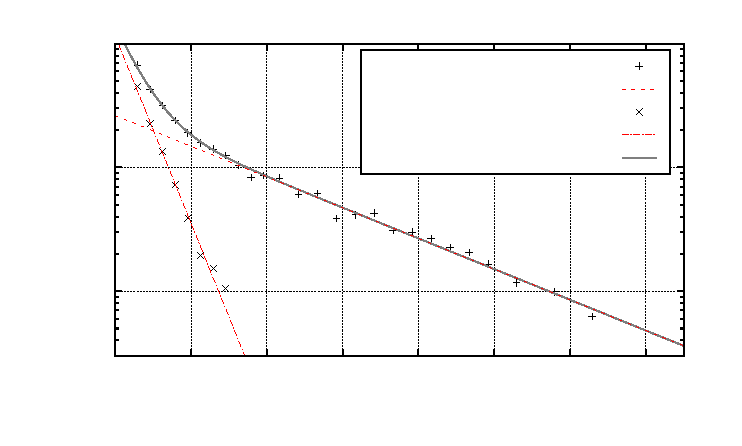
\includegraphics{dataanpassning}}%
    \gplfronttext
  \end{picture}%
\endgroup

\caption{Uppmätt och korrigerad aktivitet som funktion av tid med
  kurvanpassningar. De båda isotopernas aktivitet kan särskiljas genom
att i princip bara den ena isotopen finns kvar vid stora tider. Så en
exponentalanpassning kan göras till datan i den högra änden av
plotten. Därefter kan den kortlivade isotopens aktivitet extraheras
genom att subtrahera den första anpassingen från datan i den vänsta
änden. De anpassade havleringstiderna blev
$\Thalv{108}{Ag}=\unit[146\pm9]{s}$ och $\Thalv{110}{Ag}=\unit[23,9\pm0,9]{s}$.}
\label{fig:data}
\end{figure}

Med metoderna från avsnitt~\ref{sec:databehandling} kan de två olika halveringstidrena beräknas. Genom att sedan jämföra de erhållna halveringstidrena med de redan kända värdena~\cite{wiki_silver} kan respektive isotop kopplas till de erhållna värdena. Detta visas i \figref{fig:data}. Därifrån ses också att vi fick $\Thalv{108}{Ag}=\unit[146\pm9]{s}$ och $\Thalv{110}{Ag}=\unit[23,9\pm0,9]{s}$ (osäkerhetsgränserna är $1\sigma$).
Vi ser nu att de kända värdena på 142\,s respektive 24,6\,s ligger väl innanför felmarginalerna för våra mätningar. 

%Utan att dra ut på det för mycket kan man bara tillägga här att anpassningarna i \figref{fig:data} också ger värden på hur stor respektive isotops aktivitet var prescis när aktiveringen avslutades. Detta tillsammans med data om relativ förekomst av de två naturliga silverisotoperna kan ge information om det relativa tvärsnittet för dem.  


\section{Sammanfattning}

% \newpage
 \bibliographystyle{ieeetr}
 \bibliography{referenser}%kräver en fil som heter 'referenser.bib'          




\end{document}





%% På svenska ska citattecknet vara samma i både början och slut.
%% Använd två apostrofer (två enkelfjongar): ''.


%% Inkludera PDF-dokument
\includepdf[pages={1-}]{filnamn.pdf} %Filnamnet får INTE innehålla 'mellanslag'!

%% Figurer inkluderade som pdf-filer
\begin{figure}\centering
\centerline{ %centrerar även större bilder
\includegraphics[width=1\textwidth]{filnamn.pdf}
}
\caption{}
\label{fig:}
\end{figure}

%% Figurer inkluderade med xfigs "Combined PDF/LaTeX"
\begin{figure}\centering
\resizebox{.8\textwidth}{!}{\input{filnamn.pdf_t}}
\caption{}
\label{fig:}
\end{figure}

%% Figurer roterade 90 grader
\begin{sidewaysfigure}\centering
\centerline{ %centrerar även större bilder
\includegraphics[width=1\textwidth]{filnamn.pdf}
}
\caption{}
\label{fig:}
\end{sidewaysfigure}


%%Om man vill lägga till något i TOC
\stepcounter{section} %Till exempel en 'section'
\addcontentsline{toc}{section}{\Alph{section}\hspace{8 pt}Labblogg} 

